
\documentclass{TP}
\usepackage[utf8]{inputenc}
\usepackage{amsmath}
\usepackage{amssymb}
\usepackage[numbers]{natbib}
\usepackage{booktabs}
\usepackage{multirow}
\usepackage[raggedleft]{sidecap}   
\usepackage[english]{babel}
\usepackage{hyperref}
\usepackage[bottom]{footmisc}
%\selectlanguage{english}

\begin{document}

%====================================================
%\begin{french*}{english}
\title{Automatic lineage construction from time-lapse yeast cells images}
\author{G. Brenna\footnotemark, N. Vadot$^1$, F. Massard$^1$, S. J. Rahi\\}
%\small \textit{These autors contributed equally}
\date{\today}
\institution{EPFL \\}

\pagestyle{plain}

%===============================================

\begin{abstract}

Time-lapse microscopy is widely used in biophysical experiments because it allows to visualize activities of living cells in real time. However, cell lineage analysis is still done manually by researchers. For the model organism S. cerevisiae, developing automatic lineage tracing algorithms is a challenging task, especially when cells are densely packed together. In this paper, Bread - a program to determine automatically the lineage of yeast cells based on a sequence of microscopy images - is presented (see Source Code \cite{lien github}). Bread was developed to work on segmentations obtained from YeaZ \cite{yeaz}, the state-of-the-art convolutional neural network for segmenting yeast cells images. A graphical user interface was also developed to facilitate the generation and correction of lineages. A command line interface also exists for automated tasks. The program works well on segmentations only (> 75\% accuracy) and displays outstanding accuracy (> 98\%) when given GFP fluorescence images in addition to the segmentation.
 
\end{abstract}

\maketitle

%===============================================
\footnotetext{These authors contributed equally}

\section{Introduction}

Budding yeast is widely used as an eukariotic model organism for research in genetics, molecular biology, systems biology and biophysics. To study cellular processes, live-cell imaging experiments - where living cells are imaged over time with fluorescence or brightfield microscopy - are usually carried out. In this context, investigation of cell lineage is important for a variety of reasons, from understanding cell physiology and development of multi-cellular organisms to the study of genes. However manual construction of cell lineage is laborious, time consuming and error-prone. Linking a bud to its parent cell is especially challenging when cells are crowded (Fig. \ref{crowded}). Fluorescent tagging of proteins located at the parent-bud neck facilitates pedigree annotation but usually the huge  amount  of data still requires a considerable amount of time to be analysed manually. A method automating this procedure would greatly increase the productivity of cell lineage construction.

\begin{figure}[H]
\centering
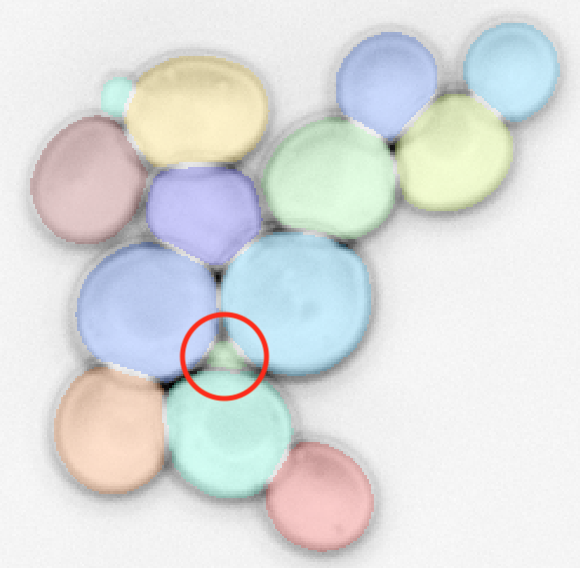
\includegraphics[width=0.76\linewidth]{Schemas et illustrations/crowded.png}
\captionsetup{justification=raggedright}
\caption{Phase contrast microscopy image of an S. cerevisiae colony segmented using YeaZ \cite{yeaz}. For the bud circled in red, identifying the parent cell is a non-trivial task.}
\label{crowded}
\end{figure}

\section{Prior work}

Previous works dedicated to the implementation of segmentation and tracking algorithms have already offered some basic tools for lineage tracing  \cite{cell-acdc} \cite{labrocca} \cite{yeastcell}. However, it was never the main focus of these works to develop fully automated lineage tracing methods. In addition, in all above-mentioned algorithms, performances without user intervention for manual correction were overall not so good and the possibility to use fluorescent markers for better prediction is not offered.
\newline So far, fully automated lineage construction algorithms have been developed only to treat data generated with cell crowding preventing devices. Such devices trap parent cells in one-ended growth chambers and progressively flush their progeny out of the chamber \cite{delta} \cite{kim} \cite{detecdiv}. Although accuracy of such algorithms are good, these programs are only useful when data is generated with aforementioned specific devices. In practice, this is very restrictive and such devices cannot always be used depending on the purpose of the study.
\newline A deep-learning-based method for tracking and lineage construction was also recently developed \cite{deepcell}. Despite having good accuracy, it has the drawback of requiring fluorescence images of cell nuclei to function which are not always available.
\newline In 2020, Kanada et al. developed a software-based analysis system to generate automatically lineage tree from time-lapse cellular images. However, their program accuracy is difficult to interpret as its efficiency given in terms of time rather than percentage. Moreover, their code is not provided making an evaluation of their program's accuracy even more difficult \cite{Kanada}.\\


In answer to above mentioned challenges, this paper presents Bread, a Python program which allows automatic lineage construction from a given set of timelapse yeast cell images (see \cite{lien github} for source code). The algorithm exploits the time-dependence between frames and can be used on segmentated brightfield or phase contrast microscopy images. When GFP fluorescence images are available, it is strongly recommended to use the GFP algorithm to achieve higher accuracy. \\

Bread was developed to work on segmentations obtained from YeaZ \cite{yeaz}, a convolutional neural network for segmenting yeast microscopy images with a graphical user interface (GUI) written in Python. YeaZ creates the segmentation masks from the time-lapse images, which are then used by Bread to generate the lineage tree.


%\newpage
%===============================================
\section{Methods}
\label{Methods}
\subsection{Segmentation analysis}
Hereunder we present lineage tracing algorithms that work using only segmentations (obtained from phase contrast or brightfield images via YeaZ) as inputs. All algorithms presented hereunder assume the movie frames are equally spaced in time.

\paragraph{Euclidean distances (ED)}
This simple algorithm uses YeaZ's segmentation masks to determine lineage relations of new buds using euclidean distances. (1) Initially, the contour pixels of every cell are extracted from the segmentation masks. (2) New buds $b$ are identified by comparing cells id's  present in the current timeframe with the ones of the previous timeframe. All other cells are identified as candidate parent cells $M_k$. (3) Then, for every possible pair of bud-parent candidate (i.e. $(b,M_k)$), the minimum euclidean distance $d_{k}$ between their contour pixels is computed. (4) Finally, the parent cell assigned to bud $b$ is the one that minimizes distances $d_{k}$. Inspiration for the conception of this algorithm was taken from \cite{cell-acdc}. Fig. \ref{fig: euclidean dist algo} visually illustrates how the algorithm works.

\begin{figure}[h]
\centering
\captionsetup{justification=raggedright}
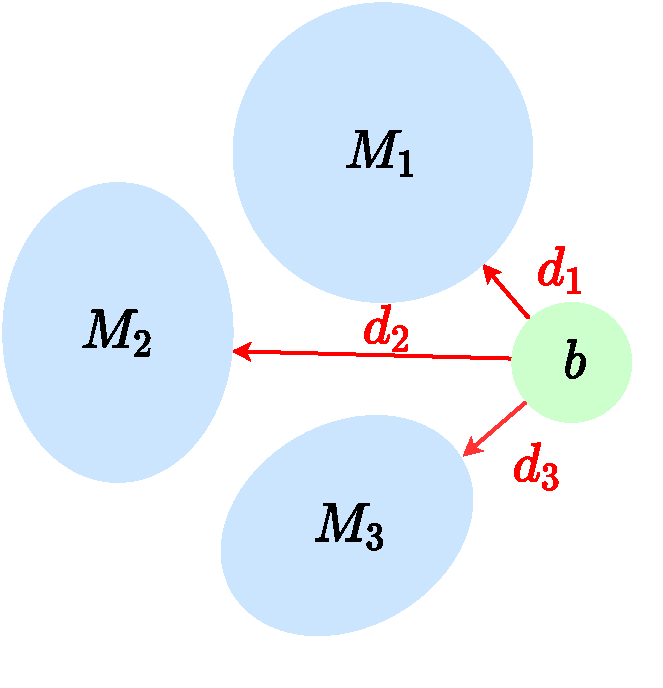
\includegraphics[width=0.7\linewidth]{Schemas et illustrations/ed.pdf}
\caption{Diagram explaining how the euclidean distances (ED) algorithm works. Cell $b_1$ corresponds to the newly detected bud and cells $M_1$, $M_2$ and $M_3$ are the candidate parent cells. Distances $d_{k}$ for $k \in [1,2,3]$ correspond to the minimal distances between the contour pixels of bud $b_1$ and the $k$-th parent candidate $M_k$. As $d_{1} < d_{2} < d_{3}$, our algorithm would assign $M_1$ as the parent of bud $b$.}
\label{fig: euclidean dist algo}
\end{figure}

\paragraph{Expansion speed (ES)} 
The intuition behind this algorithm is the simple observation that buds tend to grow away faster from their parent than from other cells. (1) We start by determining a pool of parent candidates for each emerging bud by selecting the cells located in the vicinity of the bud. This is done by computing the minimal Euclidean distance between contour pixels of the target bud and that of every other cell. Only the ones placed at a distance smaller than a specified threshold are considered as parent candidates. (2) Next, we compute the budding point $B_k$ of the target bud with respect to each parent candidate $M_k$. This is done by finding all the points on the parent's contour which are close enough to the bud (located at a distance smaller than a given threshold). If there are more than one point, we compute the average of these points, else we select the closest one. (3) Then the distance $d_k$ between the budding point $B_k$ and the point on the bud contour located furthest from the budding point is computed (see Fig. \ref{fig: expansion speed algo}). This whole step is repeated for each parent candidate $M_k$ and for $n$ successive frames $T_1,...,T_n$. (4) Then we take the numerical derivative of $d_k$ with respect to time $\frac{\Delta d_k}{\Delta t}(T_i) = \frac{d_k(T_{i+1}) - d_k(T_{i})}{T_{i+1} - T_i}$ ($i=1,...,n-1$) and we compute the arithmetic mean $X_k = \frac{1}{n-1}\sum_{i=1}^{n-1} \frac{\Delta d_k}{\Delta t}(T_i)$. (5) Finally,  the  parent  of a target bud is designated as the candidate  $M_k$  whose "expansion speed" $X_k$  is  the  maximum  of  all  the  candidates. 

\begin{figure}[h]
\centering
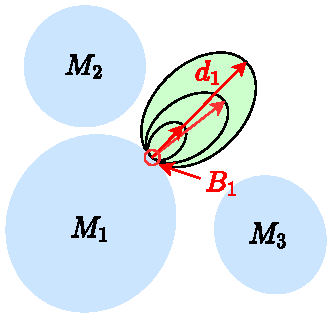
\includegraphics[width=0.7\linewidth]{Schemas et illustrations/es.pdf}
\captionsetup{justification=raggedright}
\caption{ Diagram explaining how the expansion speed (ES) algorithm works . Cells $M_k$ with $k \in [1,2,3]$ are the parent candidates to the bud (green cell). Point $B_1$ is the budding point with respect to parent candidate $M_1$. $d_1$ is the distance between the budding point $B_1$ and the point on the bud contour located furthest from it. Time evolution of $d_1$ over 3 successive timeframes is illustrated with several red arrows.}
\label{fig: expansion speed algo}
\end{figure}

\paragraph{Major axis analysis (MAA)}
This algorithm was developed after observing that new yeast daughter cells tend to grow as buds from the tip of their parent cells \cite{yeaz}. (1) Our algorithm starts by identifying new buds $b$ in a fixed timeframe $t_0$. Then, for each given timeframe $t = t_0 + j$ with $j \in \{N_{\text{offset}},...,N_{\text{offset}} + N_{\text{frames}}\}$, and for each new bud $b$, our algorithm restricts the pool of parent candidates $\{M_k (t)\}$ using the euclidian distance threshold. (2) Once the pool is selected, two features are extracted from each of the candidate cells $M_k (t)$: their major axis and the vector $\vec{v_k} (t)$ connecting their center of mass (CM) to their associated bud's one. (3) The two features are then used to compute angle $\theta_k (t)$ separating the major axis from the direction of vector $\vec{v_k} (t)$. (4) The algorithm designates the cell $M_k(t)$ with minimal $\theta_k(t)$ as the parent cell of bud $b$ in timeframe $t$ (see Fig. \ref{fig: maa algo}). (5) Finally, the parent cell of the bud is chosen using a majority vote over timeframes $t$ ranging from $t = t_0 + j$, with $j \in \{ N_{\text{offset}},...,N_{\text{offset}} + N_{\text{frames}}\}$. 
% Mathematically, it corresponds to the candidate cells that appears most frequently in the set of $\{M^{i}(t)\}$. 

Note that in this algorithm, the major axis is extracted by fitting the contour of considered cell's mask into an ellipsis. This follows from the assumption, that in general, cells seem to have an elliptic form. Additionally, number $N_{\text{offset}}$ and $N_{\text{frames}}$ are parameters of the algorithm that can be adjusted by the user. Their default value is of $N_{\text{offset}}=0$ and $N_{\text{frames}}=5$.

\begin{figure}[h]
\centering
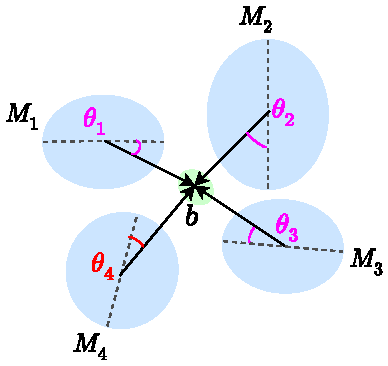
\includegraphics[width=1\linewidth]{Schemas et illustrations/maa.pdf}
\captionsetup{justification=raggedright}
\caption{ Diagram explaining how major axis analysis (MAA) algorithm works . Cells $M_k$ with $k \in [1,2,3,4]$ are the parent candidates - in timeframe $t$ - of the new bud (green cell) identified at timeframe $t_0$. Note that here $t > t_0$. $\theta_{k} $ corresponds to the angle between the major axis of $M_k$ and $\vec{v_k}$. The parent cell here is $M_4$ as it has the smallest $\theta_k$}
\label{fig: maa algo}
\end{figure}

\subsection{Fluorescence analysis (FA)} 
With this algorithms, lineage relations are guessed by looking at the budneck marker intensity along the contour of the bud.

%Offset: wait this number of frames after bud appears to look at the budneck marker channel. 

%Number of frames: number of frames to watch the budneck marker channel for. The algorithm makes a guess for each frame, then predicts a parent by majority-vote policy

(1) The first step is to compute the position of the GFP peak around the contour of the target bud. (2) Afterwards, we apply Gaussian blurring to the image. From there, the averaged luminosities in each of the bud contour points are retrieved and the pixel index of maximum luminosity is determined. (3) The next step is to find the minimum distance between the GFP peak and all other cell contours. (4) The parent of the target bud is designated as the cell closest to the GFP peak (see Fig. \ref{fig: gfp}). 

Since the budneck marker intensity is often too weak when the bud has just appeared (at time $t_0$), we wait $N_{\text{offset}}$ frames before looking at the GFP channel. Furthermore, we make a guess for $N_{\text{frames}}$ successive frames, as sometimes it takes a few frames before GFP signal reaches sufficient intensity. Therefore, our algorithm guesses a parent for each frame $t = t_0 + j$ with $j \in \{ N_{\text{offset}},...,N_{\text{offset}} + N_{\text{frames}}\}$, and then predicts the parent using majority-vote.

\begin{figure}[h]
\centering
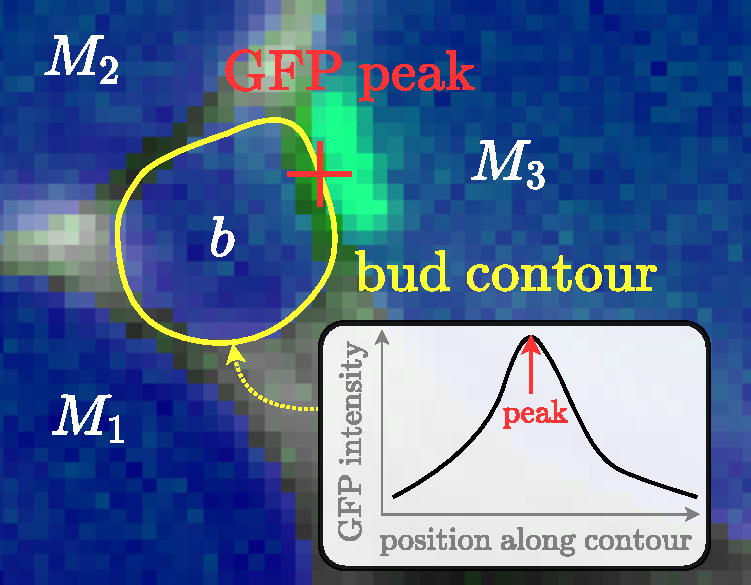
\includegraphics[width=1\linewidth]{Schemas et illustrations/fa.pdf}
\captionsetup{justification=raggedright}
\caption{The GFP luminosity is plotted along the contour of the bud in order to find the peak, and deduce the parent of the cell.}
\label{fig: gfp}
\end{figure}

\subsection{Algorithm parameters}
\label{algo param}

Different parameters can be tuned by the user to improve the overall performance of the algorithms.

First, for all algorithms, the refractory period $N_{\text{ref}}$ can be adjusted. This parameter indicates the time interval $t_{\text{ref}} = N_{\text{ref}} \cdot \Delta_t$  - with $\Delta_t$ the time separating two timeframes - during which a parent cell which had just budded cannot divide again. Therefore, immediately after budding, a parent cell is excluded from the parent pool for the next $N_{\text{ref}}$ frames.

The ES algorithm has five additional parameters which must be set: 
\begin{itemize}
\setlength\itemsep{0.0em}
\item The nearest neighbours threshold $r_{\text{nn}}$, which is the maximum distance between two cell masks's contours for them to be considered nearest neighbours. 
\item The "flexible nearest neighbour" optional parameter, that allows (when enabled) the closest cell to the bud to become a parent candidate if no nearest neighbour is found within $r_{\text{nn}}$.
\item The number of frames considered to compute the expansion velocity.
\item The "ignore nan distances" optional parameter, which, when set to True, ignores candidates for which the computed expansion speed is nan, otherwise raises an error. 
\item The max interface distance $r_{\text{max}}$, which is the maximal distance between points on the parent and bud contours for them to be included in the calculation of the budding point.
\end{itemize}

The MAA algorithm has two parameters to be adjusted in addition to the refractory period : 
\begin{itemize}
\setlength\itemsep{0.0em}
    \item The number of offset frames $N_{\text{offset}}$ we wait - after a bud appears - before guessing the parent.
    \item The number of frames $N_{\text{frames}}$ over which we make a guess after the bud has appeared. The algorithm makes a guess for each frame, then predicts the parent using a majority-vote.
\end{itemize}

The FA algorithm uses the same parameters as MAA, plus the following : 
\begin{itemize}
\setlength\itemsep{0.0em}
    \item The size of the Gaussian smoothing kernel in pixels.
    \item The number of standard deviations to consider for the smoothing kernel.
\end{itemize}

\section{Graphical user interface (GUI)}

The GUI allows to easily run the presented algorithms, load and edit lineages (csv files), and visualize results directly on top of the colony images. Multiple channels can be loaded in order to manually verify the obtained lineages. The lineage editor on the right facilitates editing by focusing the viewer on a clicked cell in the lineage file, and adding a red background for invalid cell ids (cells not present in the colony at a given time index). Special cell ids are used, -3 to indicate the absence of a guess, -2 to indicate that the cell is not a member of the colony (it was flushed into the frame from outside), -1 to indicate the cell was already here on the first frame. A screenshot of the GUI is presented in Fig. \ref{fig:gui}.

Algorithms can be run on the loaded segmentation - and GFP channel, in the case of the FA algorithm - via a wizard presented in Fig. \ref{fig:wizard}. The algorithm parameters are documented and can be manually adjusted as needed, then the computed lineage is automatically added to the lineage editor. The code is also well documented, and an example of programmatic usage is given in \cite{lien github}.


\section{Results}

\paragraph{Accuracy} To evaluate our algorithm performance, we used an accuracy metric defined as: \begin{equation*}
    \text{ACC} = \frac{\text{\# of correctly assigned buds}}{\text{total \# of buds}}
\end{equation*}

It is worth mentioning that when the algorithm is unable to determine a bud's parent (for instance, due to errors in the segmentation), the latter will not be included in the calculation of the accuracy.

The data used to evaluate our algorithms consist in 5 colonies of budding yeast, with phase contrast images taken at 5 minutes interval, for a total of 180 images per colony. For notation purposes, the $i$-th colony is referred to as $C_i$ for $i \in [1,2,3,4,5]$. The movies were segmented and tracked using YeaZ and the segmentation masks were corrected manually to avoid segmentation errors. Table \ref{tab: acc} summarizes the prediction accuracy of each algorithm for each colony.


\begin{table}[H]
\begin{tabular}{cc||c|c|c|c}
& ALGO & ED & ES & MAA & FA \\ \hline \hline
\multicolumn{1}{c|}{\multirow{6}{*}{ACC [$\%$]}} & $C_1$  &  76  &  75  & 80     &  100 \\ \cline{2-6} 
\multicolumn{1}{c|}{}                          & $C_2$  &  74  &  81  & 74     &   99  \\ \cline{2-6} 
\multicolumn{1}{c|}{}                          & $C_3$  &  61  &  73  &   68   &   99  \\ \cline{2-6} 
\multicolumn{1}{c|}{}                          & $C_4$  &  67  &  65  &   59   &   97  \\ \cline{2-6} 
\multicolumn{1}{c|}{}                          & $C_5$  &  78  & 81  &   68   &  100   \\ \cline{2-6} 
\multicolumn{1}{c|}{}                          & Mean   &  71  &  75  & 70    & 99    \\ 
\end{tabular}
\captionsetup{justification=raggedright}
\caption{Table summarising the prediction accuracy (ACC) of each implemented algorithm (see Section \ref{Methods} for more precision), namely: Euclidean distances (ED), Expansion speed (ES), Major axis analysis (MAA), Fluorescence analysis (FA). $C_i$ for $i \in [1,2,3,4,5]$ refers to the $i$-th data colony.} 
\label{tab: acc}
\end{table}

%===============================================
%\newpage
\section{Discussion}
\label{Discussion}

The simple euclidean distances and major axis analysis algorithm yield reasonable accuracy of about 71\% (see Table \ref{tab: acc}). The expansion velocity algorithm - which was implemented as an improved version of the euclidean distances algorithm - improves the prediction accuracy images by  4 percentage points on average. Considering that this brings the algorithm performance up to human accuracy levels (or even above) such results can be considered satisfactory. On the other hand, the FA algorithm achieves near perfect accuracy (> 98\%). Overall, performance measures show that, from segmented microscopy images, our algorithms are able to provide  reliable lineage predictions using very little computational time (maximum of 5s on a standard laptop, for about 180 frames containing in total about 150 budding events). This is especially useful for reducing time spent on lineage analysis and tracing, which so far is done manually by researchers. \\


The implemented algorithms also have some drawbacks. First, although in this paper segmentation masks were manually corrected for accuracy computation, some degree of arbitrariness was still involved in the process and must be taken into account when evaluating algorithm performance. 

Segmentation algorithms like ED, ES or MAA are heavily dependant on the quality of the input images's segmentation. In fact, as all three algorithms  use cell masks to make predictions, it suffices for some cells to have jagged contours in their segmentations for the predictions to change drastically. Dependency on input segmentation is even greater in the ES and MAA algorithm - compared to the ED one - as distances $d_k$, elliptic fitting and center of mass computations are made over several timeframes. For MAA in particular, performance proves to be slightly worse than the ED although the method was originally envisioned as an improvement of it. This follows as the program assumes cells to have an elliptic shape. In fact, although this hypothesis matches brightfield images observations, the masks extracted from the segmentations rarely posses smooth contours that can be fitted into an ellipsis. As a result, major axis and CM computations become inaccurate causing the algorithm performance to diminish. Segmantation algorithms  also seem to work best when new buds are detected early, namely when they are still small. This is another drawback as early bud detection is not always possible during segmentation. Finally, the ES algorithm also has the drawback of requiring at least two timeframes to make predictions. As a result, it is not possible to find lineage tracing for the buds appearing in the last frame. Overall, robustness of the segmentation algorithms to small segmentation variations is rather weak. Nonetheless, one of their advantage is that they work given any segmented image sequence, no matter the method used to generate them.

The FA algorithm doesn't have  a lot of drawbacks except for the fact that it requires additional data - recorded using the green protein fluorescence channel - to work. Indeed, depending on the subject of study, this is not always possible. Furthermore, all errors made in lineage prediction (see Table \ref{tab: acc}) can be attributed to specific cell dispositions (identified from the test sets) that induce our algorithm into error. For instance, it can happen that in very crowded environments the GFP signal of two neighbouring cells overlaps or that two parent candidates are equidistant from a GFP peak. In both situations, ambiguous cell configuration leads to incorrect predictions. Note however that, usually, situations which are problematic to the FA algorithm are also problematic for researchers who trace the lineage manually. Note also that the FA algorithm is much more robust to small segmentation variations than the segmentation ones. \\

Regarding the dependency of algorithm performance on algorithm parameters, one must state that to add a refractory period $N_{\text{ref}}$ (see Section \ref{algo param}) has no effect on improving prediction accuracy. On the contrary it seems to slightly worsen it, as with it mistakes in predictions propagate in time. As for other parameters, only the $N_{\text{frames}}$ used for majority vote guessing in and the number of frames used to compute expansion velocity have significant impact on performance. Other parameters are less sensitive to small variations around the default value. Prediction accuracies are optimal for our datasets when running programs with the latter.



%===============================================
%\newpage
\section{Conclusion}
\label{Conclusion}

We have presented Bread, a set of algorithms capable of extracting lineage relations from budding yeast cell segmentations with an accuracy greater than 75\% using segmentations only, and an accuracy greater than 98\%  when using the corresponding GFP channel \cite{lien github}. Along with the developed GUI, this program therefore enables the study of lineage properties on a large scale, greatly diminishing manual labor. The limitations of the segmentation-only algorithms (of which the expansion speed (ES) algorithm performs the best) are certainly due to the low information density and noise contained in the segmentations. Nonetheless, their performance is still satisfactory as manually tracked lineage results are not usually better, and manual tracking of lineages given only segmentations is nearly impossible.

When the GFP marker is absent, further research might use the mCherry marker as another source of information for determining lineages, where one can see DNA transfer during budding events. It should also be noted that these methods rely on segmentations obtained using external methods, and that using phase contrast directly (for instance, using machine learning methods) might contain more information.

%===============================================
%\renewcommand{\bibpreamble}{Sources vérifiées le ... :}
\begin{thebibliography}{99}

\bibitem{lien github} G. Brenna, N. Vadot, F. Massard, S. J. Rahi. Source code for Bread
\url{https://github.com/ninivert/bread}. \\
\textit{Documentation and demo at \url{https://ninivert.github.io/bread/examples/lineage/demo.html}}.

\bibitem{yeaz}
Dietler, N., Minder, M., Gligorovski, V., Economou, A.M., Joly, D.A.H.L., Sadeghi, A., Chan, C.H.M., Koziński, M., Weigert, M., Bitbol, A.-F., Rahi, S.J.. 2020. \textit{A convolutional neural network segments yeast microscopy images with high accuracy}. Nature Communications 11. doi:10.1038/s41467-020-19557-4

 
\bibitem{cell-acdc}
F. Padovani, B. Mairhörmann, P. Falter‐Braun, J. Lengefeld, K. M. Schmoller. 2021. \textit{Cell-ACDC: a user-friendly toolset embedding state-of-the-art neural networks for segmentation, tracking and cell cycle annotations of live-cell imaging data}. doi:10.1101/2021.09.28.462199
 
\bibitem{labrocca}
La Brocca, R., F. Menolascina, D. di Bernardo, and C. Sansone. 2012. \textit{Segmentation, tracking and lineage analysis of yeast cells in bright field microscopy images}. Nuovo Cimento Colloquia and Communications in Physics, 35, 5, 131-139. doi: 10.1393/ncc/i2012-11342-2

 
\bibitem{delta}
Lugagne, J.-B., Lin, H., Dunlop, M.J.. 2020. \textit{DeLTA: Automated cell segmentation, tracking, and lineage reconstruction using deep learning.}. PLOS Computational Biology 16, e1007673. doi:10.1371/journal.pcbi.1007673
 
\bibitem{yeastcell}
Salem, D., Li, Y., Xi, P., Phenix, H., Cuperlovic-Culf, M., Kaern, M.. 2020. \textit{YeastNet: Deep Learning Enabled Accurate Segmentation of Budding Yeast Cells in Bright-field Microscopy}. doi:10.1101/2020.11.30.402917

 
\bibitem{kim}
 Kim, K., Rowat, A.C., Carpenter, A.E.. 2010. \textit{Automated tracking of yeast cell lineages}. in: Proceedings of SPIE. Proceedings of SPIE. doi:10.1117/12.859770
 
\bibitem{Kanada}
Kanada, F., Ogino, Y., Yoshida, T., Oki, M.. 2020. \textit{A novel tracking and analysis system for time-lapse cell imaging of Saccharomyces cerevisiae}. Genes & Genetic Systems 95, 75–83. doi:10.1266/ggs.19-00061

\bibitem{detecdiv}
Aspert, T., Hentsch, D., Charvin, G.. 2021. \textit{DetecDiv, a generalist deep-learning platform for automated cell division tracking and survival analysis}. doi:10.1101/2021.10.05.463175

\bibitem{deepcell}
Moen, E., Borba, E., Miller, G., Schwartz, M., Bannon, D., Koe, N., Camplisson, I., Kyme, D., Pavelchek, C., Price, T., Kudo, T., Pao, E., Graf, W., Van Valen, D.. 2019. \textit{Accurate cell tracking and lineage construction in live-cell imaging experiments with deep learning}. doi:10.1101/803205

\end{thebibliography}

\appendix

\onecolumn
\newpage
\section{Appendix}
\label{annexe}
\begin{figure}[H]
\centering
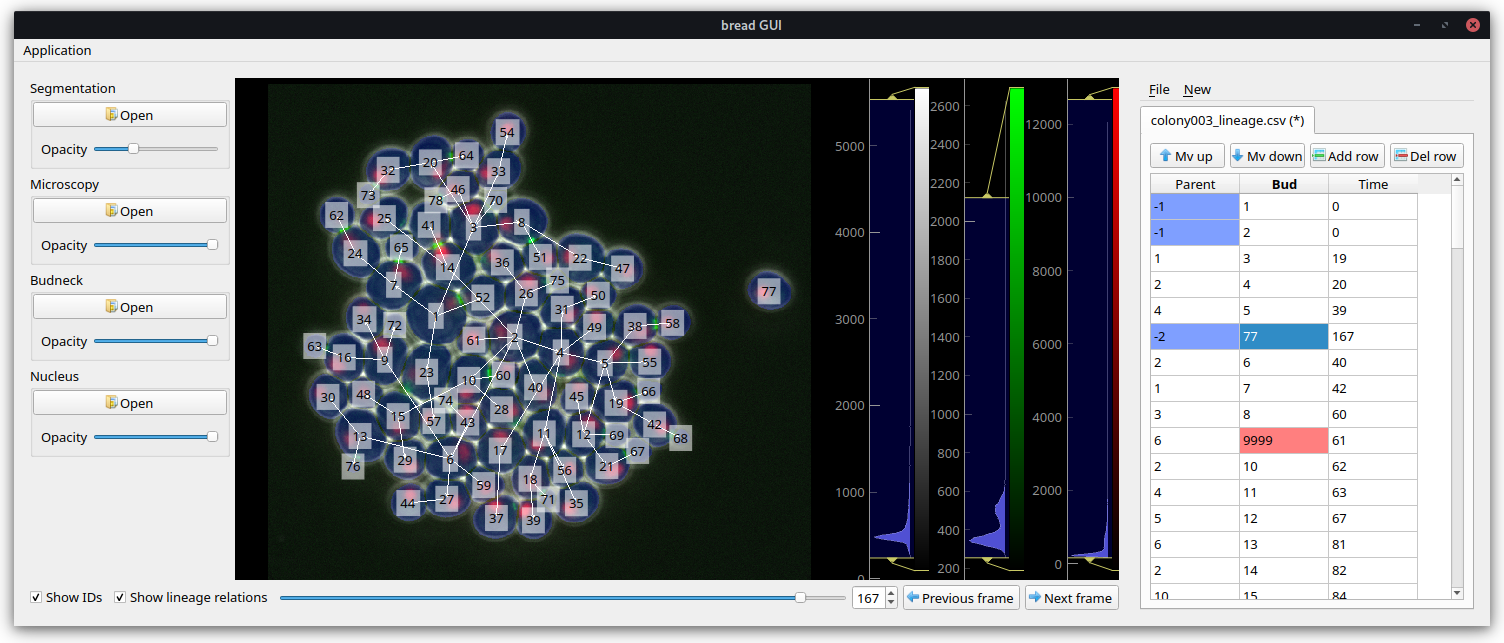
\includegraphics[width= \linewidth]{Figures/gui.png}
\captionsetup{justification=raggedright}
\caption{A screenshot of the GUI. A segmentation is loaded, as well as the corresponding phase contrast image, GFP and mCherry channels. A lineage file is loaded to the right, and the corresponding lineage relations are graphed on top of the image.}
\label{fig:gui}
\end{figure}


\begin{figure}[H]
\centering
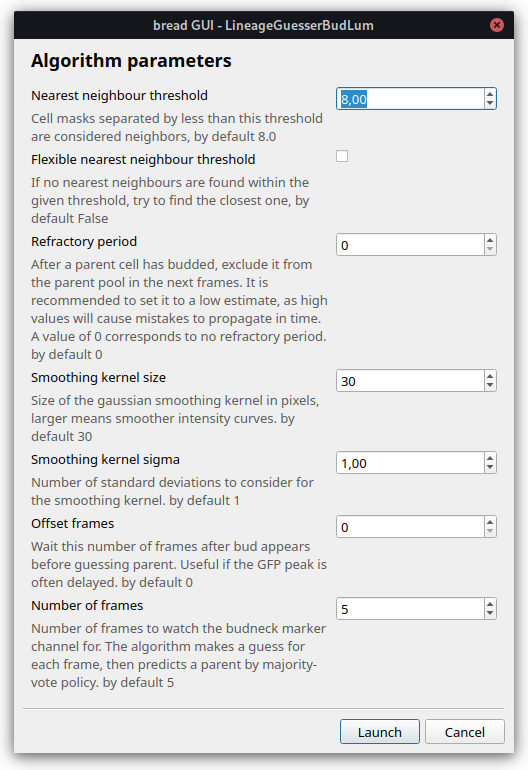
\includegraphics[width=0.5\linewidth]{Figures/param_budlum.png}
\captionsetup{justification=raggedright}
\caption{A screenshot of the parameter adjustment screen for the GFP luminosity algorithm.}
\label{fig:wizard}
\end{figure}


\end{document}

%\end{french*}
